\chapter{Data Sources, Preprocessing, and Model Contract}
\label{chap:data_model}

\section{Data Sources and Evidence Roles}
\label{sec:data_sources_evidence_roles}

This chapter defines the data sources, preprocessing assumptions, label space, model family, and runtime data contract used by the thesis pipeline. The purpose is not yet to describe the software implementation in detail; that is handled in Chapter~\ref{chap:implementation}. Instead, this chapter specifies the data and model assumptions that the offline-first architecture from Chapter~\ref{chap:architecture} must preserve.

The thesis uses multiple data sources, but each source has a different evidence role. The source-domain anxiety-related activity data provide the supervised foundation for recognizing anxiety-displaying behaviors. The Garmin-labeled user data provide the main commercial-wearable adaptation setting. The self-recorded User~7 session is kept outside training, scaler fitting, hyperparameter selection, and model selection, and is used as a blind external probe. Separate raw unlabeled Garmin sessions are used to demonstrate deployment-style pipeline execution where labels are unavailable at inference time.

\renewcommand{\arraystretch}{1.18}
\begin{table}[htbp]
\centering
\footnotesize
\caption[Data sources, evidence roles, and data scope]{Data sources, evidence roles, and data scope. Row and window counts describe preprocessing scope; performance metrics are reported in Chapter~\ref{chap:experiments}.}
\label{tab:data_sources_roles}
\begin{tabularx}{\textwidth}{p{2.6cm} p{1.4cm} p{1.7cm} p{2.4cm} X}
\toprule
\textbf{Source} & \textbf{Labels} & \textbf{Rows} & \textbf{Windows} & \textbf{Evidence role} \\
\midrule
ADAMSense \cite{khan2021adamsense}
& Labeled & 709,582 & Source-domain
& Supervised source-domain pretraining for anxiety-related or anxiety-displaying activity recognition. \\

Garmin users~1--6
& Labeled & 385,326 & 3,755 (200-sample, 100-stride)
& Fine-tuning, within-distribution validation, class-balance inspection, and user-held-out evaluation design. \\

User~7 blind probe
& Labeled & 99,017 & 989
& Blind external probe; excluded from training, scaler fitting, hyperparameter selection, and model selection. \\

25 unlabeled Garmin sessions
& Unlabeled & varies by session & 25 sessions
& Monitoring, confidence, drift, and trigger-policy demonstration at scale (Chapter~\ref{chap:experiments}); no direct accuracy claims. \\
\bottomrule
\end{tabularx}
\renewcommand{\arraystretch}{1.0}
\end{table}

These roles are enforced throughout the thesis: labeled sources support accuracy and macro-F1 claims, while the unlabeled sessions support only monitoring and trigger-policy evidence. The at-scale monitoring evaluation in Chapter~\ref{chap:experiments} covers the 25 sessions that processed successfully under the standard ingestion path.

\renewcommand{\arraystretch}{1.2}
\begin{table}[htbp]
\centering
\footnotesize
\caption[Per-source channel statistics (mean~$\pm$~standard deviation) for...]{Per-source channel statistics (mean~$\pm$~standard deviation) for the six IMU channels. Accelerometer values are in m/s$^2$ after unit normalization; gyroscope values are in deg/s. These differences are descriptive evidence of train--serve distribution shift across data sources, not model-performance evidence.}
\label{tab:channel_statistics}
\begin{tabular}{lcccccc}
\toprule
 & \multicolumn{3}{c}{\textbf{Accelerometer (m/s$^2$)}} & \multicolumn{3}{c}{\textbf{Gyroscope (deg/s)}} \\
\cmidrule(lr){2-4}\cmidrule(lr){5-7}
\textbf{Source} & $Ax$ & $Ay$ & $Az$ & $Gx$ & $Gy$ & $Gz$ \\
\midrule
ADAMSense    & $+2.22\pm5.69$ & $+0.57\pm4.89$ & $-4.49\pm3.82$ & $-0.91\pm48.46$ & $+1.73\pm23.69$ & $+0.08\pm20.97$ \\
Garmin 1--6  & $+3.22\pm6.57$ & $+1.28\pm4.35$ & $-3.53\pm3.24$ & $+0.60\pm49.93$ & $+0.23\pm14.81$ & $+0.09\pm14.17$ \\
User 7       & $+3.65\pm5.73$ & $+2.33\pm4.18$ & $-4.08\pm3.76$ & $+0.72\pm50.53$ & $+0.55\pm25.83$ & $+0.00\pm29.54$ \\
Unlabeled    & $+0.76\pm6.42$ & $+4.23\pm4.09$ & $-3.48\pm3.84$ & $+0.47\pm62.62$ & $-0.16\pm32.71$ & $+0.04\pm55.58$ \\
\bottomrule
\end{tabular}
\renewcommand{\arraystretch}{1.0}
\end{table}

\begin{figure}[htbp]
  \centering
  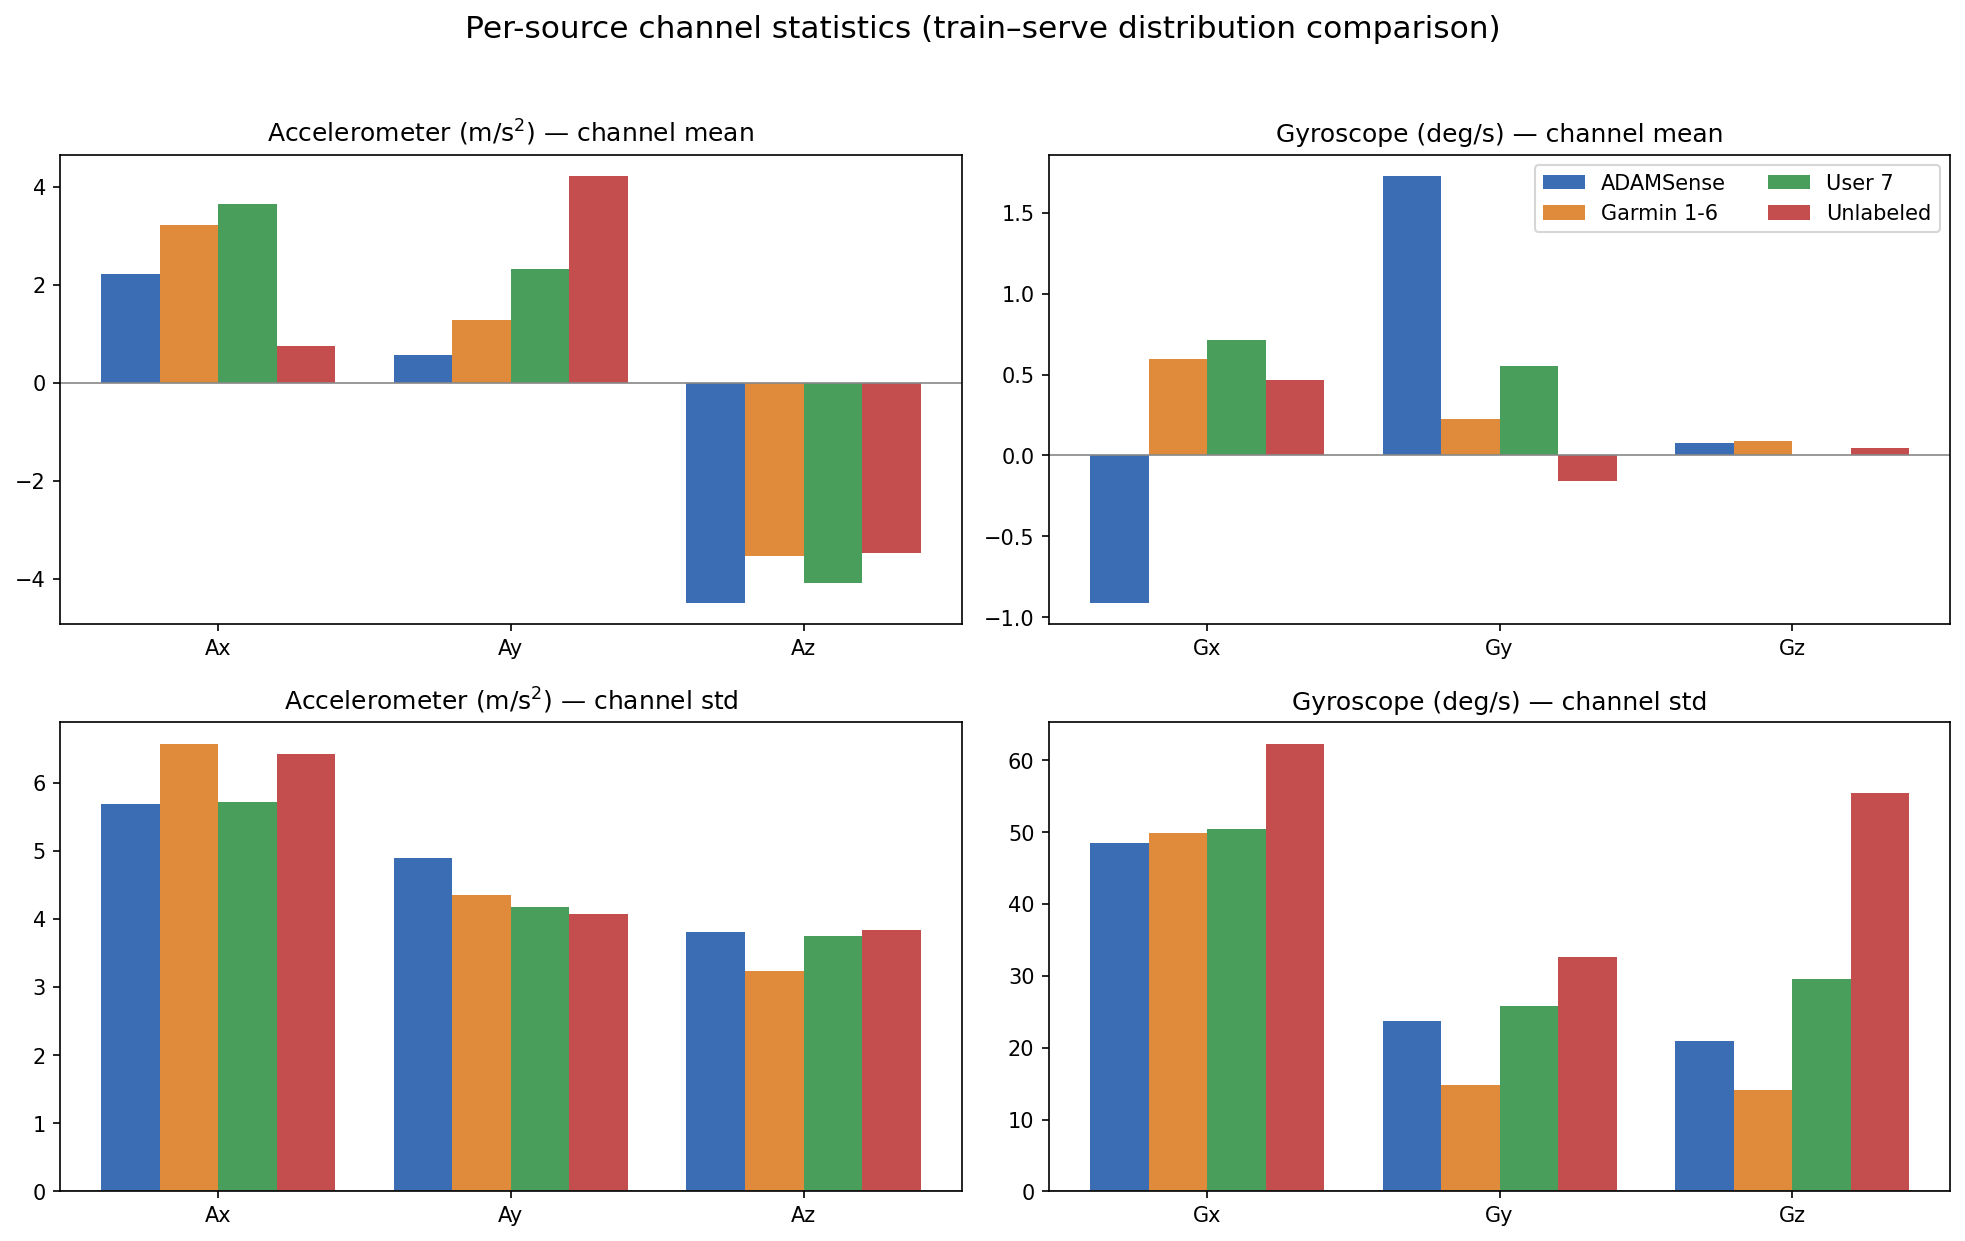
\includegraphics[width= 1\textwidth]{figures/Figure_4_1_Channel_Statistics.png}
  \caption[Per-source channel mean and standard deviation for the six IMU...]{Per-source channel mean and standard deviation for the six IMU channels after unit normalization. Differences across ADAMSense, Garmin users~1--6, User~7, and the unlabeled Garmin sessions illustrate cross-source variation relevant to train--serve distribution shift.}
  \label{fig:ch4_channel_stats}
\end{figure}
\FloatBarrier

Even at the level of unit-harmonized, unscaled channel statistics, the four sources differ in ways that matter for deployment. The unlabeled deployment-style sessions show a markedly lower $Ax$ mean ($+0.76$ vs.\ $+3.22$~m/s$^2$ for Garmin users~1--6) and a much larger gyroscope spread (for example, $Gz$ standard deviation $55.58$ vs.\ $14.17$~deg/s). These descriptive differences motivate the train--serve contract and the monitoring layer defended later, since the model must operate despite such distribution shift.

Figure~\ref{fig:ch4_magnitude} compares the accelerometer and gyroscope magnitude distributions across the four sources; the differing spreads and tails illustrate the cross-source distribution shift that the runtime contract and monitoring layer must tolerate.

\begin{figure}[htbp]
  \centering
  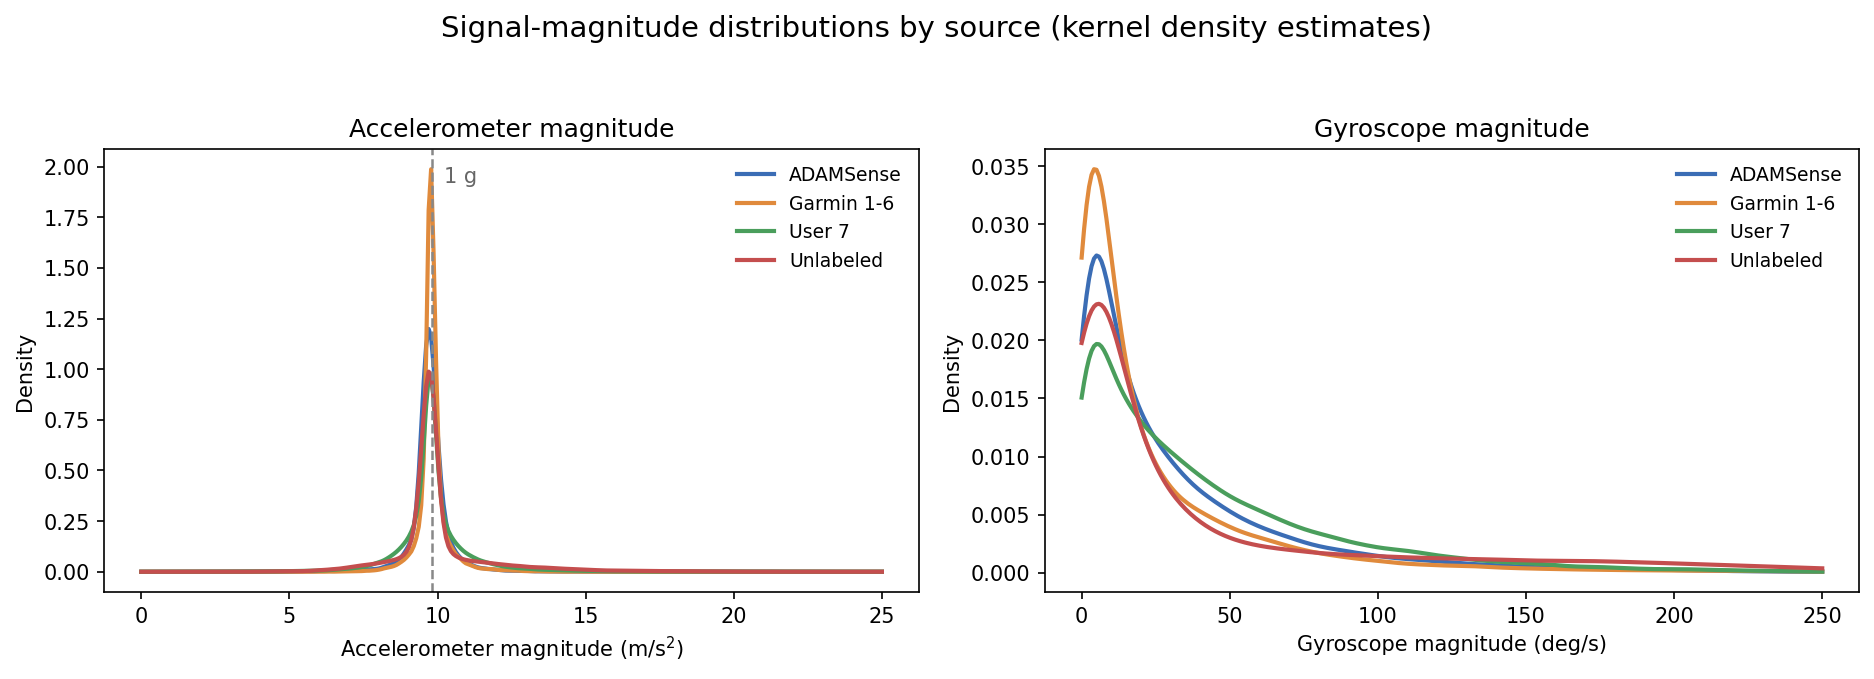
\includegraphics[width=\textwidth]{figures/Figure_4_6_magnitude_hist.png}
  \caption[Accelerometer and gyroscope signal-magnitude distributions by...]{Accelerometer and gyroscope signal-magnitude distributions by source (kernel density estimates). The accelerometer magnitude concentrates near gravity for all sources, while the peak heights and gyroscope tails differ, illustrating cross-source distribution shift.}
  \label{fig:ch4_magnitude}
\end{figure}
\FloatBarrier

The Garmin users~1--6 recordings originate from the supervisor's published data-collection study~\cite{oleh2025recognition}, collected with participant consent, while the User~7 session and the unlabeled deployment-style sessions were recorded by the author on the author's own device; no third-party personal data is introduced by this thesis. Wrist-worn HAR is sensitive to individual movement style, watch placement, and recording context~\cite{stisen2015smart,wang2024enhancing}, which is why provenance matters for interpreting the cross-user results in Chapter~\ref{chap:experiments}. The corpus is usable for controlled model development and contract verification, but it remains small and user-limited; broad population-level generalization is not claimed.

The activity classes are also imbalanced. Figure~\ref{fig:ch4_class_dist} shows the per-class window counts for Garmin users~1--6, which vary widely across the eleven activities. This imbalance is the reason macro-F1 is reported alongside accuracy and balanced class weights are used during training, as discussed in Chapters~\ref{chap:implementation} and~\ref{chap:experiments}.

\begin{figure}[htbp]
  \centering
  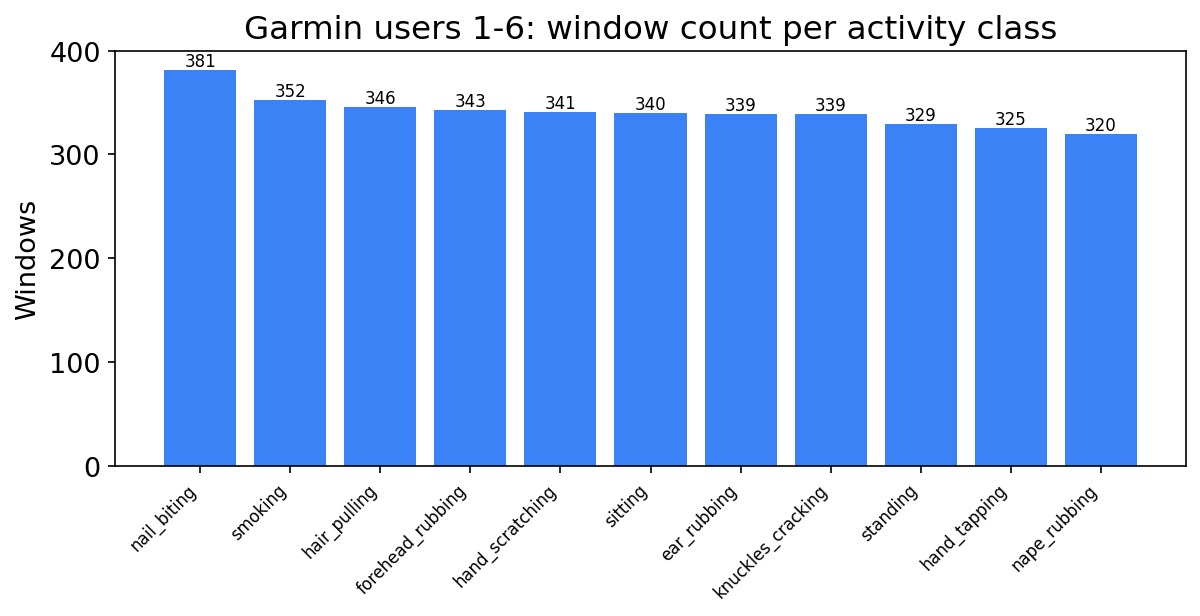
\includegraphics[width=0.92\textwidth]{figures/Figure_4_4_class_distribution.png}
  \caption[Window count per activity class for Garmin users~1--6 (3{,}755...]{Window count per activity class for Garmin users~1--6 (3{,}755 windows total). The classes are imbalanced, which motivates macro-F1 reporting and balanced class weighting.}
  \label{fig:ch4_class_dist}
\end{figure}
\FloatBarrier

\section{Sensor Schema, Units, and Label Space}
\label{sec:sensor_schema_units_label_space}

The runtime pipeline is built around a fixed six-channel inertial measurement unit schema. The canonical feature order is:

\[
Ax, Ay, Az, Gx, Gy, Gz.
\]

Here, \(Ax\), \(Ay\), and \(Az\) denote the three accelerometer axes, and \(Gx\), \(Gy\), and \(Gz\) denote the three gyroscope axes. The accelerometer channels are represented in m/s$^2$, and the gyroscope channels are represented in deg/s. This schema is treated as part of the model contract rather than as a flexible implementation detail. Any change in column order, units, or channel count changes the meaning of the input tensor and can invalidate inference.

The raw data sources do not all arrive in the same unit convention. In particular, some accelerometer recordings are represented in milli-g rather than m/s$^2$. Therefore, accelerometer unit conversion is handled before scaling and before window construction. The conversion constant used in the pipeline is:

\[
1~\text{milli-g} = 0.00980665~\text{m/s}^2.
\]

Unit conventions differ by source: the raw Garmin replay files are stored in milli-g and converted as above, whereas the source-domain ADAMSense accelerometer values are recorded in $g$ and harmonized separately into the common m/s$^2$ convention. This harmonization is applied before any cross-source statistic is computed, so that the channel comparison in Table~\ref{tab:channel_statistics} reflects genuine distribution differences rather than a unit mismatch.

Figure~\ref{fig:ch4_preprocessing_pipeline} summarizes the preprocessing contract from raw wearable data to model-ready tensors.

\begin{figure}[htbp]
  \centering
  \includegraphics[width=\textwidth]{figures/Figure_4_2_Preprocessing_Window_Construction.pdf}
  \caption[Preprocessing contract from raw wearable recordings to model-ready...]{Preprocessing contract from raw wearable recordings to model-ready tensors. Unit conversion, canonical column ordering, scaler application, and window construction are treated as contract steps rather than optional preprocessing choices.}
  \label{fig:ch4_preprocessing_pipeline}
\end{figure}

The proposed model uses only the six IMU channels \(Ax, Ay, Az, Gx, Gy, Gz\). It does not use an additional magnitude feature channel. Any reference to magnitude-scaling in the training workflow refers to training-time data augmentation, not to an extra model input feature.

The target label space contains eleven activity classes. The numeric order is fixed because the final softmax layer emits probabilities in this exact order. Table~\ref{tab:label_order} defines the mapping used by the thesis pipeline.

\renewcommand{\arraystretch}{1.2}
\begin{table}[htbp]
\centering
\footnotesize
\caption[Fixed activity-label order used by the proposed model's runtime contract.]{Fixed activity-label order used by the proposed model's runtime contract.}
\label{tab:label_order}
\begin{tabular}{cl}
\toprule
\textbf{Index} & \textbf{Activity label} \\
\midrule
0  & \texttt{ear\_rubbing} \\
1  & \texttt{forehead\_rubbing} \\
2  & \texttt{hair\_pulling} \\
3  & \texttt{hand\_scratching} \\
4  & \texttt{hand\_tapping} \\
5  & \texttt{knuckles\_cracking} \\
6  & \texttt{nail\_biting} \\
7  & \texttt{nape\_rubbing} \\
8  & \texttt{sitting} \\
9  & \texttt{smoking} \\
10 & \texttt{standing} \\
\bottomrule
\end{tabular}
\renewcommand{\arraystretch}{1.0}
\end{table}

The label order is therefore not a cosmetic metadata field. If the label file, training code, inference code, and reporting code use different orders, the model can output numerically valid probabilities that are semantically assigned to the wrong classes. For this reason, the fixed label order is part of the runtime contract and is promoted together with the trained model and preprocessing artifacts.

\section{Windowing and Tensor Representation}
\label{sec:windowing_tensor_representation}

The model operates on fixed-length time windows. After unit normalization and column ordering, the continuous six-channel time series is transformed into overlapping windows of 200 samples, following the standard sliding-window formulation of sensor-based HAR~\cite{bao2004activity,bulling2014tutorial}. At the thesis sampling rate of 50~Hz, this corresponds to a four-second input segment. The baseline stride is 100 samples, corresponding to a two-second shift between adjacent windows.

Each model input is therefore represented as:

\[
\mathbf{X} \in \mathbb{R}^{200 \times 6}.
\]

The first dimension represents time, and the second dimension represents the fixed sensor-channel order. This time-major representation is used consistently across model training, validation, and inference.

\renewcommand{\arraystretch}{1.15}
\begin{table}[htbp]
\centering
\footnotesize
\caption[Windowing and tensor contract used by the proposed model.]{Windowing and tensor contract used by the proposed model.}
\label{tab:windowing_contract}
\begin{tabularx}{\textwidth}{p{3.7cm} X}
\toprule
\textbf{Contract element} & \textbf{Value / rule} \\
\midrule
Sampling rate & 50~Hz after preprocessing and resampling. \\
Window length & 200 samples, corresponding to four seconds at 50~Hz. \\
Stride & 100 samples, corresponding to two seconds at 50~Hz. \\
Input tensor shape & \((200,6)\), with time as the first dimension and sensor channels as the second dimension. \\
Channel order & \(Ax, Ay, Az, Gx, Gy, Gz\). \\
Boundary rule & Windows are constructed within user and activity segments; a window never crosses a labeled activity boundary or a participant boundary, which avoids mixed-label windows at transitions. \\
\bottomrule
\end{tabularx}
\renewcommand{\arraystretch}{1.0}
\end{table}

The four-second window is an engineering compromise. It is long enough to contain short repetitive wrist movements such as rubbing, tapping, scratching, and biting, while remaining short enough to sustain the two-second prediction cadence of the 50\%-overlap windowing. Compared with the ADAMSense study, which reported its strongest configuration with longer 12-second windows and a magnitude feature, this thesis uses a shorter four-second window and a fixed six-channel IMU input \cite{khan2021adamsense}. This choice reduces temporal context but better matches the short-cadence offline wearable pipeline evaluated in this thesis; the windowing ablation of Section~\ref{sec:ch7_ablation} quantifies the trade.

Tensor shape alone does not guarantee temporal equivalence. A shape of \((200,6)\) states that the model receives 200 time steps and six channels, but it does not prove that two datasets share the same temporal scale, unit convention, or sampling behavior. The runtime contract therefore requires the correct upstream assumptions as well: unit conversion, sampling rate, channel order, scaler usage, and label order.

\section{Model Family and Proposed Architecture}
\label{sec:model_family_d1_architecture}

The thesis uses a one-dimensional convolutional and bidirectional recurrent neural-network family for sensor-based HAR. This model family is suitable for multichannel time-series classification because convolutional layers can extract short local motion patterns, while recurrent layers can model temporal dependencies across the input window \cite{ordonez2016deep,hammerla2016deep,kim2023tutorial1dcnnbilstm}. Long Short-Term Memory networks were introduced to address vanishing-gradient limitations in recurrent sequence learning \cite{hochreiter1997lstm}, and bidirectional recurrent layers process the sequence in both temporal directions \cite{schuster1997bilstm}.

The proposed model keeps this general 1D-CNN--BiLSTM structure. Its preprocessing and windowing configuration was selected among the candidates evaluated during development (the windowing ablation of Section~\ref{sec:ch7_ablation} reports the surviving sweep), and the resulting runtime was then frozen and promoted under that configuration. The architecture is treated as part of the experimental model family, while the exact deployed model is treated as part of the runtime contract. Model~D1 is the internal artifact name used in the repository; in the thesis text, the same runtime is referred to as the proposed model. Figure~\ref{fig:ch4_d1_architecture} summarizes the block-level design.

\begin{figure}[htbp]
  \centering
  \includegraphics[width=\textwidth]{figures/Figure_4_3_Model_Architecture_Overview.pdf}
  \caption[Block-level architecture of the proposed model]{Block-level architecture of the proposed model. The model receives a \((200,6)\) IMU window, extracts local temporal patterns using one-dimensional convolutional layers, models sequence context with bidirectional LSTM layers, and produces an eleven-class softmax output.}
  \label{fig:ch4_d1_architecture}
\end{figure}

\renewcommand{\arraystretch}{1.15}
\begin{table}[htbp]
\centering
\footnotesize
\caption[Block-level summary of the proposed model's architecture.]{Block-level summary of the proposed model's architecture.}
\label{tab:d1_architecture_summary}
\begin{tabularx}{\textwidth}{p{3.3cm} p{3.4cm} X}
\toprule
\textbf{Block} & \textbf{Role} & \textbf{Contract relevance} \\
\midrule
Input layer
& Accepts \((200,6)\) IMU windows
& Fixes the expected temporal length and six-channel sensor schema. \\

1D convolutional feature extraction
& Learns local temporal motion patterns
& Encodes short-range wrist-motion signatures from the fixed input channels. \\

Pooling / regularization
& Reduces temporal resolution and limits overfitting
& Supports more stable representation learning on limited user-level data. \\

Bidirectional LSTM layers
& Models temporal dependencies across the window
& Allows the classifier to use sequence context from both directions within the fixed offline window. \\

Dense classification head
& Maps learned representation to class probabilities
& Produces an eleven-class softmax vector in the fixed label order from Table~\ref{tab:label_order}. \\
\bottomrule
\end{tabularx}
\renewcommand{\arraystretch}{1.0}
\end{table}

The proposed model contains 967,499 parameters (966,347 trainable, 1,152 non-trainable), as verified from the build notebook output and recorded in \path{model_param_count.json} in the runtime contract folder. These counts describe architectural scale only and are not performance claims. Note that \path{model_contract.json} also records a 94.41\% pre-augmentation hold-out accuracy from the build notebook; this uses a single 10\% stratified split executed during training and is distinct from the rigorous post-hoc five-fold cross-validation result of 93.61\% reported in Chapter~\ref{chap:experiments}. Recognition results, cross-validation scores, and blind-probe behavior are reported later in Chapter~\ref{chap:experiments}.

The architecture is intentionally not presented as a clinical detector. It is a sensor-based activity-recognition model for behaviors that may be relevant to anxiety-related monitoring. The model predicts activity classes from wearable IMU windows; any interpretation beyond activity recognition must be handled carefully and is outside the direct model output.

\section{Runtime Data and Model Contract}
\label{sec:runtime_data_model_contract}

The central operational assumption of this chapter is that the trained model is not deployable as an isolated file. The model only has a valid meaning together with its preprocessing rules, scaler, label order, input shape, and monitoring baseline. This thesis therefore treats the deployed unit as a runtime contract rather than as a standalone neural-network checkpoint.

Formally, the deployed unit is the runtime contract
\[
\mathcal{C}=(M,\,S,\,L,\,B,\,\Omega),
\]
where $M$ is the frozen model, $S$ the train-only scaler, $L$ the fixed label order, $B$ the monitoring baseline, and $\Omega$ the preprocessing and windowing metadata (unit convention, channel order, window size, and stride). The scaler $S$ applies the per-channel standardization
\[
x'_{i,j}=\frac{x_{i,j}-\mu_j}{\sigma_j},\qquad j\in\{Ax,Ay,Az,Gx,Gy,Gz\},
\]
where the mean $\mu_j$ and standard deviation $\sigma_j$ are fitted only on the Garmin training data (users~1--6) and are never recomputed from User~7 or production sessions. Reusing the saved $\mu_j$ and $\sigma_j$ is what preserves the train--serve feature space; fitting a fresh scaler on an incoming batch would silently change the input distribution the model was trained on.

\renewcommand{\arraystretch}{1.15}
\begin{table}[H]
\centering
\footnotesize
\caption[Runtime data and model contract for the thesis pipeline.]{Runtime data and model contract for the thesis pipeline.}
\label{tab:runtime_contract_summary}
\begin{tabularx}{\textwidth}{p{3.5cm} X}
\toprule
\textbf{Contract item} & \textbf{Required rule} \\
\midrule
Model checkpoint
& The promoted model file is used for inference. It must not be swapped independently from the scaler, label order, and monitoring baseline. \\

Input shape
& Every inference batch must contain windows of shape \((200,6)\). \\

Channel order
& The six input channels must be ordered as \(Ax, Ay, Az, Gx, Gy, Gz\). \\

Accelerometer unit
& Accelerometer values must be represented in m/s$^2$ before scaler transformation. Milli-g inputs must be converted using \(1~\text{milli-g}=0.00980665~\text{m/s}^2\). \\

Gyroscope unit
& Gyroscope values are represented in deg/s. \\

Scaler
& The saved Garmin train-only scaler is applied at inference. A new scaler must not be fitted on production or probe data. \\

Windowing
& Windows use 200 samples and 100-sample stride after preprocessing. Labeled windows must not cross activity boundaries. \\

Label order
& Softmax outputs are decoded using the fixed eleven-class label order in Table~\ref{tab:label_order}. \\

Monitoring baseline
& Drift and confidence checks are interpreted relative to the promoted baseline that belongs to the same runtime contract. \\

Evidence boundary
& Labeled data can support supervised metrics. Unlabeled deployment-style data can support monitoring and trigger-policy evidence, but not direct accuracy claims. \\
\bottomrule
\end{tabularx}
\renewcommand{\arraystretch}{1.0}
\end{table}
\FloatBarrier

This contract avoids a common deployment failure mode in which a model checkpoint is updated without also updating the preprocessing artifacts that give the input tensor its meaning. For example, applying a different scaler, reordering the sensor channels, or decoding the softmax vector with a different label list may not produce a runtime error, but it can silently change the semantics of the prediction. In the thesis pipeline, this is treated as an MLOps problem rather than a purely modeling problem.

The same contract also protects the interpretation of monitoring. A drift alert is meaningful only if it is computed in the same feature space and with the same preprocessing assumptions as the model input. Therefore, the scaler, monitoring baseline, model checkpoint, and label-order file must be promoted together. This same-folder invariant is developed as an implementation rule in Chapter~\ref{chap:implementation}.

\section{Chapter Summary}
\label{sec:chapter4_summary}

This chapter defined the data and model assumptions that the offline-first MLOps pipeline must preserve. The data sources were separated by evidence role, spanning source-domain supervised pretraining data, labeled Garmin development data, blind labeled User~7 probe data, and unlabeled deployment-style Garmin data, and the chapter then fixed the six-channel IMU schema, unit assumptions, label order, windowing procedure, and model family. The central point is that the proposed model is not only a neural-network checkpoint but part of a runtime contract that also binds unit conversion, channel order, scaler usage, label decoding, window construction, and monitoring baselines into a single deployable unit. These assumptions are what make the later evaluation and monitoring results interpretable. Performance metrics are intentionally deferred to Chapter~\ref{chap:experiments}, while this chapter establishes the evidence boundaries and deployment contract needed to interpret those results safely.
